\documentclass[12pt]{article}
\usepackage{graphicx}
\usepackage{float}

\topmargin 0.0cm
\oddsidemargin 0.2cm
\textwidth 16cm 
\textheight 21cm
\footskip 1.0cm

\title{Project Milestone}
\author{Zach Stecher}
\date{Due: 11/15/16}

\begin{document}

\maketitle

\section*{\centering{Abstract}}

I discuss the problem of solving image-based classification using readily available machine learning techniques. Specifically, I discuss the issue of accurately classifying 99 species of plants using binary leaf images with multiple features. For this project I compare the results achieved by different available algorithms to find the most effective solution, and discuss real world applications and ease of practical use. In this paper I discuss my experiences with KNeighbor, Linear Discriminant Analysis, and Random Forest.

\section{Introduction}

 The focus of this paper is the problem of leaf classification, which was posted as a competition for the data science site Kaggle.com. Results for the competition were scored based on the Logarithmic Loss of the submission csv file. The objective was to submit a prediction set that achieved a log loss as close to zero as possible. Participants were provided with the leaf pictures as well as a training data file and a test data file in csv form, but not the answers for the test data. While this is generally regarded as a simple problem to solve using existing standard techniques, there is always opportunity to expand our understanding of existing problems and techniques by applying and comparing them..

\subsection{Practical Application}

Automated plant recognition as a subset of general image based classification has a multitude of real world applications. Beyond just the academic implications, an accurate classifier open to the public could aid in applications like medicinal research, species tracking, agricultural research, medicinal practice in low-income countries where manufactured pharmaceutical solutions are not available, and much more.

\subsection{Related Work}

The classification problem is possibly the oldest in machine learning, yet still continues to present new and interesting challenges to the community. In 2003, Koby Crammer and Yoram Singer explored the problem of ranking topics for text documents, often referred to as a \textit{multi-label} classification problem. The end goal for Crammer and Singer was to be able to predict topic relevance of documents based on their content where each document may be associated with \textit{multiple} relevant topics, and rank the relevance of each topic. While not an exact mirror of the Leaf Classification problem I attempt to tackle in this paper as each leaf will only have one right answer, the submission requires probabilities adding up to 100 percent, so multiple classifications may be assigned based on how sure the algorithm is of its answer. Crammer and Singer also encounter the problem of filtering out irrelevant information from their sample documents to avoid causing errors through including incorrect features or data. This is a very similar problem to one I encountered while trying to predict plant species, as some leaves may share certain features exactly but differ on others to the point where including the exact matching features would only serve to cloud the results. Feature selection and filtering ended up being a significant barrier in both papers.

A less obvious facet of the Leaf Classification problem is the issue of associating images with text that does not describe the image, or is difficult to infer from the image, such as labeling a leaf with the name of a species. Fortunately this issue was explored in 2003 (Barnard et al., 2003). They described the issue as one of \textbf{annotation} and \textbf{correspondence}, with annotation referring to predicting using all inforation present and correspondence associating particular words with particular image substructures. This matches relatively well with the issue in Leaf Classification of feature filtering. For example, perhaps differentiating two leaves by the number of points at their tips as a seperate layer from the entire shape of the leaf, or its texture. We end up with a prediction based on a large collection of correspondence.

\section{Methodology}

Because the point of this project was to identify the most effective way to tackle the leaf classification problem, I decided the most prudent way to start would be to test out various readily available classifiers to see if one existed that was up to the task, or could at least provide a solid jumping off point. To accomplish this, I looked through the keernals posted by others on the Kaggle competition page for this problem, and was lucky enough to find that someone had already put together a program running and comparing ten different common classifiers. At first glance three classifiers stood out from the rest:

\begin{figure}[H]
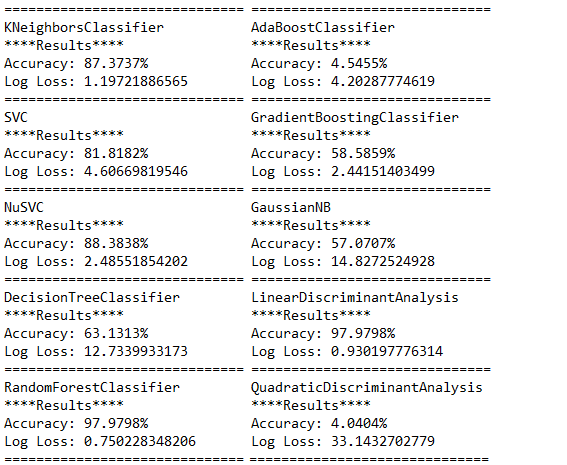
\includegraphics{ClassifierComparison.png}
\caption{Initial Classifier Results}
\end{figure}

It's apparent that Linear Discriminant Analysis(LDA), KNeighbor, and Random Forest are the three most accurate classifiers with their standard parameters set, with Random Forest providing the best score of the three. Before moving forward, I wanted to see if there were any way to improve KNeighbor or LDA to the point that they could overtake Random Forest's initial score. After several tries adjusting the parameters, I was unable to improve either score to the point where continuing with them over Random Forest made sense. I had also intended to include TensorFlow, Google's open source machine learning library. Unfortunately unforseen technical restrictions prevented me from doing so during this specific project. I had also attempted to utilize Theano as a substitute for TensorFlow, but this was derailed by technical difficulties as well. As a result, for the remainder of this project I worked with Random Forest.

Because the version of Random Forest included with the classifier comparison was very basic, I decided to implement a newer version that would allow for full parameter manipulation without the restriction of having to also work with 9 other classifiers.The focus from this point was to fine tune the parameters to attempt to beat the default score. This new implementation also opened the possibility of ranking the available features by relevance, should I decide to limit which ones are available to the model during training and testing.

\subsection{Results}

After fine tuning the parameters on the Random Forest model, I was able to achieve a best LogLoss score of 0.67886 with 100 trees.  Any attempt with less than 100 trees would result in a significantly higher LogLoss, while the difference between 100 trees and up to 500 trees was minimal, with LogLoss beginning to creep up slightly after that. Interestingly, when ranking the available features the vast majority of them came out to be relatively equal in importance. Only two stood out as significantly more important than the average, while less than ten were determined to be of little importance. This leads me to conclude that the vast majority of these features are important in classifying \textbf{some} of the leaf samples, but only one or two were useful in classifying nearly \textbf{all} of them, while a small number were either not useful at all or only useful in a few fringe cases. Because of the high number of features and the nature of image classification, it seems necessary to be able to account for a large number of similarities while looking for the sometimes subtle differences in order to make a choice. Random Forest appears to be a good starting point for this process, as it's nature as an ensemble model that `votes' and provides a consensus answer makes it resistant to providing answers based on irrelevant features, yet still account for those features during a different data point where they may be useful. It's very adept at tackling problems that require consideration on a case by case basis.

\section{Conclusion}

In this paper I attempted to tackle the problem of Leaf Classification as presented by the competition hosted by Kaggle. After trying out a variety of classifiers and identifying three front runners, I attempted to bring the second and third place models in line with the front runner to ensure I would not be prematurely eliminating a valid model. Once unable to do so I was confident moving forward with Random Forest and it did not fail to provide some valuable insight into the nature of this classification problem and some of the bigger issues faced when attempting to solve it. The ability to score and rank features provided by Random Forest made it apparent that a problem such as this requires a model with the ability to consider different combinations of features on a case-by-case basis. To this end I would continue this line of thought by employing some more advanced models such as TensorFlow or other multi-layered neural networks to achieve a higher level of accuracy.

\clearpage

\section{Appendix}

\begin{figure}[H]
    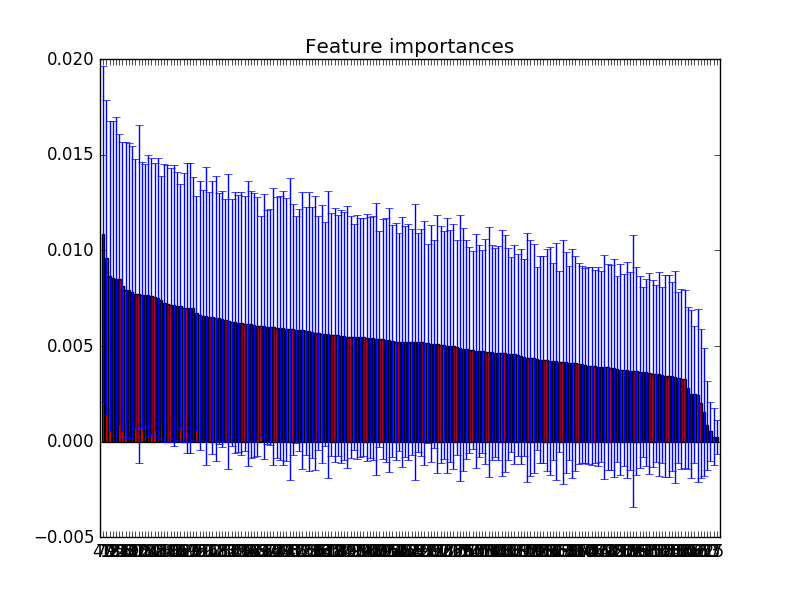
\includegraphics[scale=0.9]{featureImportance.png}
    \caption{Plotted Feature Importance}
\end{figure}

\begin{figure}[H]
    \centering
    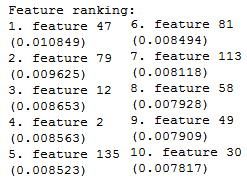
\includegraphics{FeatureRanking.png}
    \caption{Top 10 Features}
\end{figure}

\section{References}
\begin{itemize}
	\item K. Crammer and Y. Singer. A Family of Additive Online Algorithms for Category Ranking. In \textit{Journal of Machine Learning Research 3} (2003) 1025-1058
	\item K. Barnard, P. Duygulu, D. Forsyth, N. de Freitas, D. M. Blei, and Michael I. Jordan. Matching Words and Pictures. In \textit{Journal of Machine Learning Research 3} (2003) 1107-1135
	\item The Kaggle Competition: https://www.kaggle.com/c/leaf-classification
	\item Iinitial classifier comparison code and information: https://www.kaggle.com/jeffd23/leaf-classification/10-classifier-showdown-in-scikit-learn
	\item Initial Random Forest implementation: https://www.kaggle.com/sunnyrain/leaf-classification/random-forests-with-0-68-score
	\item https://www.tensorflow.org/
	\item http://deeplearning.net/software/theano/
\end{itemize}


\end{document}